\documentclass[12pt, a4paper]{article}
\usepackage[spanish]{babel}
\selectlanguage{spanish}
\usepackage[utf8]{inputenc}
\usepackage{booktabs}%tablas
\usepackage{caption,threeparttable}%Alinear titulo izquierda
\captionsetup{justification   = raggedright,singlelinecheck = off}
\usepackage[font=small,labelfont=bf]{caption}%%%%%%%%% caption
\usepackage{graphicx}
\usepackage{float} %Ubicacion Tablas
\usepackage{multirow}%tablas
\usepackage{lscape} %pag horizontal
%\usepackage[spanish,activeacute,es-tabla]{babel}
\usepackage[T1]{fontenc}
%\usepackage[latin1]{inputenc}
\usepackage{setspace}
\usepackage[usenames]{color}
\usepackage{apacite}
\setlength{\parindent}{3em}%sangria el em es espacio
\usepackage{geometry}
\geometry{top=4cm,bottom=4cm,left=4cm,right=2.4cm}% Margenes
\usepackage{natbib}
\begin{document}
\begin{titlepage}
\begin{center}
\textbf{Implementación de una linea de producción de muebles en la empresa Servimaderas de la ciudad de Cuenca.}\\%negrita
\vspace{0.5cm}
\vspace{3cm}
Trabajo de titulación presentado como requisito para optar al título de \\
\vspace{0.5cm}

\textbf {MASTER EN GESTION DE PROYECTOS}\\

\vspace{2cm}
Por los estudiantes\\
\vspace{0.5cm}

\textbf {Marco Antonio CALLE ROJAS}\\
\vspace{1cm}
\textbf{Andrea Carolina GORDILLO SILVA}\\
\vspace{3cm}
Bajo la dirección de:\\
\vspace{1cm}
Alfredo Armijos, PMP\\
\vspace{3cm}
ESPAE Escuela de Postgrado en Administración de Empresas\\
Maestría en Gestión de Proyectos\\
Guayaquil-Ecuador\\

AÑO\\

2017
\end{center}
\end{titlepage}

%%%%%%%%%%%%%%%%%%%%%%%%%%%%%%%%%%%%%%%%%fin portada
\tableofcontents%INDICE
\listoftables%INDICE de tablas
\listoffigures% Indice figuras

\doublespace %para doble espacio lineas
\setlength{\parskip}{\baselineskip}% espacio párrafo 
\bibliographystyle{apalike}

%%%%%%%%%%%%%%%%%%%%%%%%%%%%%%%%%%%%%%%%%%%%%
% ESPACIO DE ITEMS
\let\olditemize\itemize
\def\itemize{\olditemize\itemsep=0pt }
%%%%%%%%%%%%%%%%%%%%%%%%%%%%%%%%%%%%%%%%%%
\newpage

\section {Entorno Institucional}
\subsection{Introducción General}
\subsubsection{Hitos Institucionales}

La empresa ``SERVIMADERA'' se encuentra a las afueras de la ciudad de Cuenca en la parroquia Portete de Tarqui siendo su actividad principal la fabricación de partes y piezas de madera para empresas dedicas a la industria del mueble. Dentro de su cartera de clientes se  encuentran las empresas mas grandes de muebles del Azuay así como pequeñas empresas que fabrican muebles de forma artesanal.

La empresa nació hace 10 años como un aserradero  de madera  en el cual trabajaban 5 personas en un terreno arrendado.   En el año 2012 compró un terreno donde actualmente funciona la empresa y agregó nuevos equipos teniendo un incremento  constante en su gama de productos y servicios; ademas  ha incrementado su plantilla de colaboradores a 16 personas.

\subsubsection{Contexto Nacional}
La empresa `SERVIMADERA'' posee una infraestructura  que le permite crecer e incursionar en nuevos mercados; ademas la experiencia de su grupo humano genera que sus productos tengan acogida dentro del cantón . 


\subsubsection{Contexto Internacional}
La empresa actualmente no cuenta con presencia internacional.

\subsubsection{Gobierno Corporativo}
La empresa posee dos lineas principales de negocio que son:
\begin{itemize}
	\item Producción de partes y pieza de madera
	\item Servicio de secado de madera
\end{itemize}

Los cuales son el nivel operativo de la cadena de valor. En su nivel de estrategia se tiene la parte administrativa que esta compuesta por:
\begin{itemize}
\item Gerencia General
\end{itemize}
Entre las áreas de soporte no se incluye ninguna ya que los servicios que se requieren son realizados por terceros.
\subsubsection{Desafíos Institucionales}
La empresa ``SERVIMADERA'' tiene varios desafíos tanto internos como externos basados en las  debilidades y amenazas entre las que se encuentran.
\begin{itemize}
	\item Incremento de productos sustitutos a la madera para la fabricación de muebles, disponibles en el mercado como el plástico y el metal.
	\item Contracción del mercado nacional en un 4,5\% según proyecciones del FMI para el 2017.
	\item Proyecciones de crecimiento económico para el Ecuador negativas de  -1.6 \% por el FMI y -1.3\% por el Banco Mundial.
	\item No existen procesos estándar para la elaboración de muebles en la empresa lo que provoca  reducción en la eficiencia de producción.
	\item La ausencia de control en los procesos existentes   produce un alto porcentaje de desperdicio en las  material primas.
	\item Equipos y espacios de fabricación subutilizados al tener una producción menor a capacidad de su planta.
	\item Los canal de comunicación utilizados actualmente no permiten realizar un seguimiento a los clientes para conocer su grado de satisfacción con los productos.
\end{itemize}
	
\subsection{Filosofía Institucional}
\subsubsection{Misión}
Producir y comercializar soluciones en madera y complementos para la industria del mueble  orientados a generar valor para la comunidad en la que desarrollamos nuestras actividades
\subsubsection{Visión}
Ser una empresa líder a nivel regional en la fabricación y comercialización de productos, piezas e insumos de madera para la industria y un referente de excelencia empresarial.

\subsubsection{Valores}
Los valores que la empresa SERVIMADERAS están enfocados a cumplir con sus clientes y sus colaboradores en cada uno de sus productos siendo estos:
\begin{itemize}
	\item Orientación al cliente: Buscamos ofrecer soluciones a nuestros clientes, satisfaciendo sus necesidades y superando sus expectativas.
	\item Trabajo en equipo: Valoramos el trabajo en equipo, escuchamos las opiniones de otros para fortalecer el trabajo que realizamos.
	\item Mejora continua: Brindar un servicio en constante mejora conlleva a un servicio de excelencia.

   
Alianzas estratégicas: Creamos sinergia con otros para lograr la excelencia en el servicio.
Responsabilidad social: Tenemos un compromiso con la comunidad y el me- dio ambiente.

\subsection{Modelo de Negocio (BMC)}	
\subsubsection{Segmento de Mercado}
El mercado actual de la empresa Servimaderas es el sector industrial de la fabricación de muebles en la ciudad de Cuenca . El 70\% de la producción  que realiza mensualmente es vendida a un único cliente que es el mas grande productor de muebles a nivel nacional. El resto de su producción se distribuye entre dos empresas de menor tamaño y productores artesanales. Siendo su único mercado la parte sur del Ecuador específicamente Azuay.
\subsubsection{Propuesta de Valor}
La propuesta de valor de la empresa Servimaderas es ofrecer partes y piezas para la producción de muebles de alta calidad según los requerimientos sus clientes mediante el uso de equipo que permite producir cualquier tamaño de elemento solicitado ; con el uso de materia prima que han pasado por un proceso de secado para garantizar la durabilidad de sus productos.
\subsubsection{Relación con los Clientes}
Dentro de la empresa existe una relación con sus clientes internos y externos debido a las características del negocio. La relación con sus clientes externos es a través de conversaciones telefónicas y el uso de correo electrónico. Estos medios son comúnmente usados para recibir pedido o reclamos por parte del cliente externo. Al momento de realizar las entregas el personal de reparto  recibe cualquier feedback que el cliente indique.

\subsubsection{Canales de Servicio}

El principal canal de servicio es a través de la atención  telefónica de una secretaria que cumple la función de asesor comercial permitiendo un comunicación directa con el cliente que se transforma una comunicación rápida. Dentro de la empresa se usa el correo electrónico como un medio para confirmar pedidos y fechas de entrega.

\subsubsection{Actividades Clave}
\begin{itemize}
	\item  Adquisición de la materia prima que se obtiene de bosques principalmente de Esmeraldas
	\item  Transporte de los tablones
	\item  Recepción y almacenamiento de los tablones
	\item  Secado de la madera en un horno
	\item  Proceso de producción de partes y piezas según requerimiento del cliente
	\item  Entrega de  productos al clientes
\end{itemize}
\subsubsection{Recursos Claves}
Dentro de los recursos claves con los que cuenta la empresa para el desarrollo del negocio se tienen los siguientes:
\begin{itemize}
	\item Vehículos propios para entrega de productos
	\item Equipo de protección personal para sus colaboradores.
	\item Equipo humano calificado para las labores
	\item Infraestructura adecuada para la fabricación de sus productos.
\end{itemize}
\subsubsection{Alianzas Claves}
La alianza principal se forma con los proveedores los cuales se encuentran en las siguientes áreas.
\begin {itemize}
	\item Proveedores de materias primas que son varios y se encuentran principalmente en la provincia de Esmeraldas.
	\item Proveedores de mantenimiento principalmente de mantenimiento correctivos de los equipos de la empresa.
	\item Proveedores de equipo de seguridad y ropa de trabajo.
\end{itemize}
\subsubsection{Estructura de Costos}
Los costos que la empresa tiene comúnmente viene dados de la siguiente forma:
\begin {itemize}
	\item \textbf {Costos Variables}
		\begin {itemize}
			\item Sueldo y aportaciones al IESS de los trabajadores	
			\item Pagos a Proveedores 
			\item Mantenimiento correctivo
			\end{itemize}

\end{itemize}		
	\item \textbf {Costos Fijos}
		\begin {itemize}
			\item Servicios Básicos
			\item Mantenimiento preventivo e infraestructura
			\item Suministros 
			\end{itemize}
		\end{itemize}
\subsubsection{Estructura de Ingresos}

Los ingresos de la compañía se encuentran formados los 2 servicios   que ofrece a sus clientes, los cuales  depende de la gestión de cobranzas siendo estos servicios:
\begin {itemize}
	\item Venta  de partes y piezas de madera para armado de muebles.
	\item Servicio de secado de madera.
\end{itemize}

\subsection{Estrategia Institucional}
\subsubsection{Estrategia General}
Para cumplir con la misión y visión establecidas por la empresa se ha definido una estrategia general de crecimiento enfocada a diversificación de productos y creación de valor para el cliente.La estrategia se sustenta en  4 pilares fundamentales que son :
\begin{itemize}
	\item  Asegurar un crecimiento sostenible 
	\item  Apertura de nuevos mercados
	 \item Asegurar procesos productivos eficientes
	\item Asegurar colaboradores de alto desempeño
\end{itemize}

Con el fin de establecer la relación entre los pilares de la estrategia general con los objetivos estratégicos que se persiguen y sus estrategias se presenta esta relación en la Tabla \ref{Estrategia General} la cual indica ademas la perspectiva de la estrategia en función del cuadro de mando integral.


\begin{table}[H]

\centering


\caption  {\textit{Estrategia General }}


\label{Estrategia General}
\begin{tabular}{|p{2.5cm}|p{4cm}|p{4.5cm}|p{2.5cm}|}
\hline
\textbf{Pilares Estratégicos} & \textbf{Objetivos Estratégicos} & \textbf{Estrategias} & \textbf{Perspectiva} \\ \hline
\multirow{2}{2.5cm}{\\ Asegurar un crecimiento sostenible} & \multirow{2}{4.5cm}{\\Control de gastos  e incremento de ingresos en un 10\%.} & Monitoreo de los costos de operación en todas las áreas de la empresa & Financiera \\ \cline{3-4} 
 &  & Incrementar el volumen de ventas de productos y servicios. & Financiera \\ \hline
\multirow{2}{2.5cm}{\\Apertura de nuevos mercados} & \multirow{2}{4.2cm}{Expandir participación en el mercado de la costa en un 10 \% mediante el desarrollo de un plan comercial} & Oferta de nuevos productos a nuevos segmentos de mercado. & Mercado \\ \cline{3-4} 
 &  & Incrementar la satisfacción de los clientes & Mercado \\ \hline
\multirow{2}{2.5cm}{\\Asegurar procesos productivos eficientes} & \multirow{2}{4cm}{Incrementar la eficiencia en el proceso productivo en un 7\% y reducir desperdicios en un 2\%} & Reducir tiempos de producción y estandarizar procesos. & Procesos internos \\ \cline{3-4} 
 &  & Capacitar a los colaboradores en técnicas de mejora continua & Aprendizaje y Conocimiento \\ \hline
\multirow{3}{2.5cm}{\\Asegurar colaboradores de alto desempeño} & \multirow{3}{4cm}{\\Desarrollar al personal potenciando los valores de profesionalismo y calidad} & Contar con colaboradores con conocimiento de mantenimiento preventivo & Aprendizaje y Conocimiento \\ \cline{3-4} 
 &  & Establecer métodos de reconocimiento y recompensa para generar motivación & Aprendizaje y Conocimiento \\ \cline{3-4} 
 &  & Establecer métodos de evaluación de desempeño. & Aprendizaje y Conocimiento \\ \hline

\end{tabular}

\end{table}


\subsubsection{Matriz de correlación}

Las diferentes estrategias revisadas se las analiza y relaciona entre si para establecer la matriz de relaciones que permite obtener un criterio más objetivo de relaciones de estrategias.

Se propone la siguiente calificación en función de su relación: 


\begin{itemize}	
	\item Alta Relación 	= 	3
	\item Media Relación = 	2
	\item Baja Relación 	= 	1
\end{itemize}

En la Tabla \ref{tabla:2} se puede revisar el resultado de las relaciones existentes entre las diferentes estrategias establecidas.\\


\begin{table}[H]
\centering
\caption{\textit{Matriz de correlaciones}}
\label{tabla:2}
\begin{tabular}{|p{1.4cm}|p{6cm}|p{0.4cm}|p{0.4cm}|p{0.4cm}|p{0.4cm}|p{0.4cm}|p{0.4cm}|p{0.4cm}|p{0.4cm}|p{0.4cm}|}
\hline
\textbf{Código} & \textbf{Estrategias} & \textbf{E1} & \textbf{E2} & \textbf{E3} & \textbf{E4} & \textbf{E5} & \textbf{E6} & \textbf{E7} & \textbf{E8} & \textbf{E9} \\ \hline
\textbf{E1} & Monitoreo de los costos de operación en todas las áreas de la empresa &  &  &  &  &  &  &  &  &  \\ \hline
\textbf{E2} & Incrementar el volumen de ventas de productos y servicios. & 1 &  &  &  &  &  &  &  &  \\ \hline
\textbf{E3} & Oferta de nuevos productos a nuevos segmentos de mercado. & 1 & 2 &  &  &  &  &  &  &  \\ \hline
\textbf{E4} & Incrementar la satisfacción de los clientes & 2 & 3 & 2 &  &  &  &  &  &  \\ \hline
\textbf{E5} & Reducir tiempos de producción y estandarizar procesos. & 3 & 1 & 2 & 2 &  &  &  &  &  \\ \hline
\textbf{E6} & Capacitar a los colaboradores en técnicas de mejora continua & 3 & 2 & 1 & 2 & 3 &  &  &  &  \\ \hline
\textbf{E7} & Contar con colaboradores con conocimiento de mantenimiento preventivo & 2 & 1 & 1 & 1 & 3 & 1 &  &  &  \\ \hline
\textbf{E8} & Establecer métodos de reconocimiento y recompensa para generar motivación & 2 & 1 & 1 & 1 & 3 & 2 & 2 &  &  \\ \hline
\textbf{E9} & Establecer métodos de evaluación de desempeño. & 3 & 1 & 1 & 2 & 3 & 2 & 2 & 2 &  \\ \hline
\end{tabular}
\end{table}


\subsubsection{Mapa Estratégico}

\begin{figure}[H]
  \centering
  
    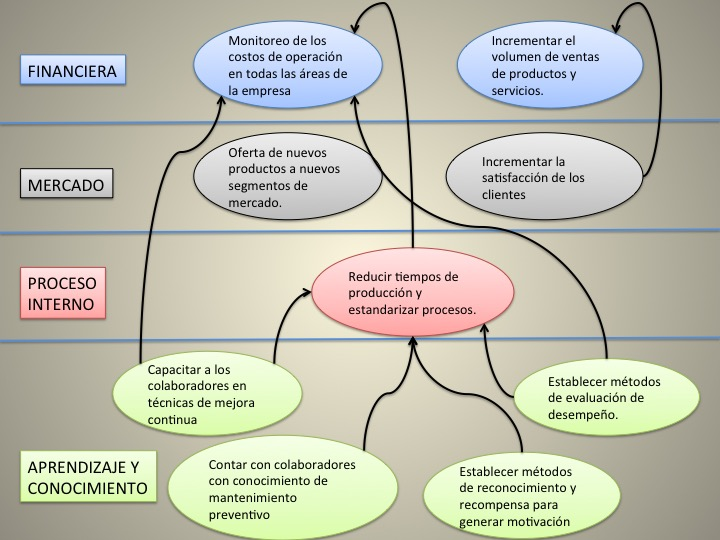
\includegraphics[width=1.1\textwidth]{Diapositiva1.jpg}
  \captionsetup{justification=centering} %Centrar caption 
  \caption{Mapa Estratégico}
  \label{figura:1}
\end{figure}

%%%%%%%%%%%
\subsection{Cuadro de Mando Integral}
\subsubsection{Perspectiva Financiera}
	\begin{itemize}	
	\item Monitoreo de los costos de operación en todas las áreas de la empresa

	\item  Incrementar el volumen de ventas en productos y servicios

\end{itemize}

\subsubsection{Perspectiva de Mercado}
	\begin{itemize}	
		\item Oferta de nuevos productos a nuevos segmentos de mercado

		\item Incrementar la satisfacción de los clientes
	\end{itemize}
	
	\subsubsection{Perspectiva de Procesos Internos}
	\begin{itemize}	
	\item Reducir tiempos de producción y estandarizar procesos
		\end{itemize}
		
	\subsubsection{Perspectiva de Aprendizaje y Experiencia}
	\begin{itemize}	
		\item Capacitar a los colaboradores en técnicas de mejora continua
		\item Contar con colaboradores con conocimiento de mantenimiento preventivo
		\item Establecer métodos de reconocimiento y recompensa para generar motivación
		\item Establecer métodos de evaluación de desempeño
	\end{itemize}
	
	\subsection{Despliegue de Perspectivas}
	\subsubsection{Objetivos Financieros}
	\begin{itemize}	
		\item Reducir los costos de operación en todas las áreas de la empresa en un 5\%
		\item Incrementar el volumen de ventas en productos y servicios en un 10\% mediante la diversificación de mercado de los productos elaborados.
	\end{itemize}
	
	
	\subsubsection{Objetivos de Mercado}
	\begin{itemize}	
		\item Incrementar la participación en el mercado de la costa en un 10\% mediante el desarrollo de un plan comercial y la promoción de nuevos productos y servicios en las ciudades de Guayaquil, Manta y Machala.
		\item Incrementar la participación de mercado en un 15\% en la zona sur del austro mediante la implementación de una sección de diseño
		\item Incrementar la satisfacción de los clientes mediante la reducción del 1\% del número de reclamos por fallas. 
	\end{itemize}
	
		\subsubsection{Objetivos de Procesos Internos}
	\begin{itemize}	
		\item Incrementar la productividad en un 20\% mediante la renovación de equipos obsoletos y mejora de procesos 
		\item Implementar una sección de diseño para reducir tiempos de fabricación en un 15\% y estandarizar el proceso de trabajo para reducir desperdicios en un 20\% en un plazo de 1 año.
		
	\end{itemize}
	
	\subsubsection{Objetivos de Aprendizaje y Conocimiento}
	\begin{itemize}	
		\item Capacitar a los colaboradores en técnicas de mejora continua
		\item Contar con colaboradores con conocimiento de mantenimiento preventivo
		\item Establecer métodos de reconocimiento y recompensa para generar motivación
		\item Establecer métodos de evaluación de desempeño
	\end{itemize}
\subsubsection{Despliegue de perspectivas}

En la Tabla \ref{tabla:3} se desarrollan los indicadores de desempeño y su meta, correspondiente a los objetivos estratégicos para cada perspectiva.
	
\begin{table}[H]
\centering
\caption{\textit{{Despliegue de perspectivas}}}
\label{tabla:3}
\begin{tabular}{|p{2.5cm}|p{4.9cm}|p{4.6cm}|p{1cm}|p{1cm}|}
\hline
\textbf{Perspectiva} & \multicolumn{1}{c|}{\textbf{Objetivos}} & \multicolumn{1}{c|}{\textbf{Indicadores (KPIs)}} & \textbf{Valor actual} & \textbf{Meta} \\ \hline
\multirow{2}{2cm}{\textbf{Financiera}} & Reducir  costos de operación en todas las áreas en un 5\% & Ahorro anual de costos & 1\% & 5\% \\ \cline{2-5} 
 & Incrementar el volumen de ventas en  10\% mediante la diversificación de mercado . & Incremento de ventas en relación al año anterior & 3\% & 10\% \\ \hline
\multirow{3}{5cm}{\textbf{Mercado}} & Incrementar la participación en el mercado de la costa en  10\% mediante  un plan comercial y  promoción  en las ciudades de Guayaquil, Manta y Machala. & Incremento de participación de mercado de la costa en relación al año anterior & 5\% & 10\% \\ \cline{2-5} 
 & Incrementar la participación de mercado en un 15\% en la zona sur del austro  & Incremento de participación de mercado en la zona sur del austro en relación al año anterior & 5\% & 15\% \\ \cline{2-5} 
 & Incrementar la satisfacción de los clientes mediante la reducción del 1\% del número de reclamos por fallas. & Porcentaje de reducción de reclamos por fallas & N/a & 1\% \\ \hline
\multirow{3}{3cm}{\textbf{Procesos Internos}} & Incrementar la productividad en un 20\% mediante mejora de procesos & Porcentaje de incremento de productos terminados en relación al año anterior & 5\% & 20\% \\ \cline{2-5} 
 & \multirow{2}{4.7cm}{Implementar una sección control de procesos para optimizar tiempos en un 15\% } & Reducción de tiempo de fabricación & 0\% & 15\% \\ \cline{3-5} 
 &  & Reducción de desperdicios & 0\% & 20\% \\ \hline
\multirow{4}{2.2cm}{\textbf{Aprendizaje y conocimiento}} & Capacitar a los colaboradores en técnicas de mejora continua & Porcentaje de cumplimiento de planes de capacitación & 0\% & 100\% \\ \cline{2-5} 
 & Contar con colaboradores con conocimiento de mantenimiento preventivo & Porcentaje de colaboradores con conocimiento de mantenimiento preventivo & 0\% & 50\% \\ \cline{2-5} 
 & Establecer métodos de reconocimiento y recompensa  & Porcentaje de métodos establecidos & 0\% & 100\% \\ \cline{2-5} 
 & Establecer métodos de evaluación de desempeño & Porcentaje de métodos establecidos & 0\% & 100\% \\ \hline
\end{tabular}
\end{table}

\subsubsection{Iniciativas}
A partir de las metas establecidas en la Tabla \ref{tabla:3} se han establecido tres iniciativas para conseguir las metas establecidas.

\begin{table}[H]
\centering
\caption{\textit{Iniciativa}}
\label{Iniciativas}
\begin{tabular}{|p{3.2cm}|p{6cm}|p{4.5cm}|}
\hline
\textbf{Perspectiva} & \textbf{Objetivos} & \textbf{Iniciativas} \\ \hline
\textbf{Financiera} & Incrementar el volumen de ventas en 10 \% mediante la diversificación de mercado & \multirow{3}{4.5cm}{\\Implementar una producción eficiente mediante diversificación de portafolio y apertura de nuevos mercados}\\ \cline{1-2}
\textbf{Mercado} & Incrementar la participación en el mercado de la costa en 10\% mediante un plan comercial y promoción en las ciudades de Guayaquil, Manta y Machala. &  \\ \cline{1-2}
\textbf{Mercado} & Incrementar la participación de mercado en un 15 \% en la zona sur del austro &  \\ \hline
\textbf{Mercado} & Incrementar la satisfacción de los clientes mediante la reducción del 1 \% del número de reclamos por fallas. & Establecer sistema de control de reclamos \\ \hline
\textbf{Procesos Internos} & Implementar una sección control de procesos para optimizar tiempos en un 15\% & \multirow{5}{4.5cm}{\\Implementar procesos estandarizados de producción} \\ \cline{1-2}
\textbf{Procesos Internos} & Incrementar la productividad en un 20\% mediante mejora de procesos &  \\ \cline{1-2}
\textbf{Financiera} & Reducir costos de operación en todas las áreas en un 5 \% &  \\ \cline{1-2}
\textbf{Aprendizaje y conocimiento} & Capacitar a los colaboradores en técnicas de mejora continua &  \\ \cline{1-2}
\textbf{Aprendizaje y conocimiento} & Contar con colaboradores con conocimiento de mantenimiento preventivo &  \\ \hline
\textbf{Aprendizaje y conocimiento} & Establecer métodos de reconocimiento y recompensa & \multirow{2}{4cm}{Realizar procesos de evaluación al personal} \\ \cline{1-2}
\textbf{Aprendizaje y conocimiento} & Establecer métodos de evaluación de desempeño &  \\ \hline
\end{tabular}
\end{table}



%%%%%%%%%%%
\subsection{Arquitectura Empresarial }
\begin{table}[H]
\centering
\caption{\textit{{Matriz de Arquitectura}}}
\label{Matriz:Arquitectura}
\begin{tabular}{|p{2cm}|p{3.5cm}|p{4cm}|p{4cm}|}
\hline
\multicolumn{1}{|p{2.5cm}|}{\textbf{Macro procesos}} & \textbf{Recepción de materia prima} & \textbf{Producción} & \textbf{Distribución producto terminado} \\ \hline
\multirow{4}{2.5cm}{\textbf{Personas}} & Estibador & Operadores Cortadoras & Chofer \\ \cline{2-4} 
 & Gerente & Lijadores & Ayudante \\ \cline{2-4} 
 &  & Secretaria & Estibador \\ \cline{2-4} 
 &  & Estibadores &  \\ \hline
\multirow{5}{2.5cm}{\textbf{Maquinaria}} & Tecles manuales & Cortadoras de madera & Camión \\ \cline{2-4} 
 & Horno de secado & Lijadoras & tecle manual \\ \cline{2-4} 
 &  & Pistolas neumáticas & Embaladora \\ \cline{2-4} 
 &  & Compresores &  \\ \cline{2-4} 
 &  & Cierras cinta &  \\ \hline
\multirow{4}{2.5cm}{\textbf{Información}} & Orden de Compra & Hojas de control inventario & Facturas \\ \cline{2-4} 
 & Guías de remisión & Orden de producción & Guía de recorrido \\ \cline{2-4} 
 &  & Hojas de despacho & Detalle de entrega \\ \cline{2-4} 
 &  & Hojas de control de calidad &  \\ \hline
\multicolumn{1}{|p{2.5cm}|}{\textbf{Servicios y Productos}} & Recepción de productos & Producción de productos & Entrega de productos \\ \hline
\multirow{4}{2cm}{\textbf{Regulaciones}} & Ley de Gestión ambiental(Ministerio del Ambiente) & Reglamento de seguridad y salud de los trabajadores y mejoramiento del medio ambiente de trabajo & Reglamento de seguridad y salud de los trabajadores y mejoramiento del medio ambiente de trabajo \\ \cline{2-4} 
 & Permisos de funcionamiento y bomberos & Código del Trabajo de Ecuador & Código del Trabajo de Ecuador \\ \cline{2-4} 
 & Reglamento de Seguridad y Salud de trabajadores(Ministerio de trabajo) &  & Ley de Gestión ambiental(Ministerio del Ambiente) \\ \cline{2-4} 
 & Registro Único de Contribuyente(RUC) &  & Ley Orgánica de Transporte Terrestre, Tránsito y Seguridad Vial (ANT) \\ \hline
\end{tabular}
\end{table}


\subsubsection{Cadena de Valor}
\begin{figure}[H]
  \centering
  
    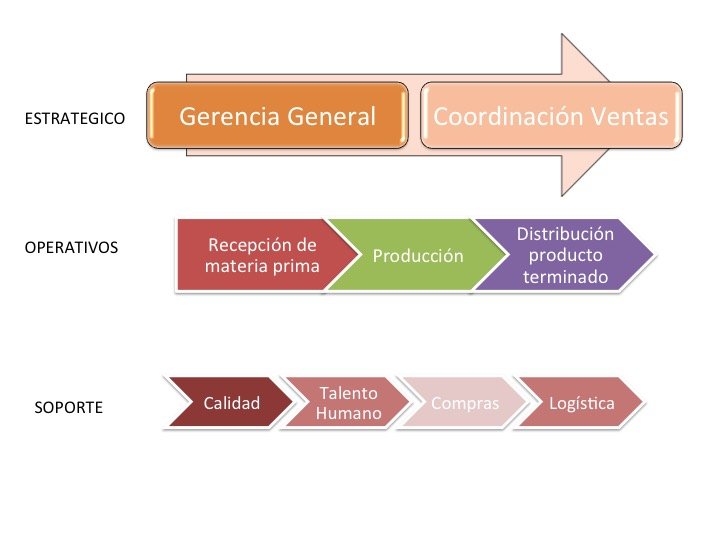
\includegraphics[width=1.1\textwidth]{CadenadeValor.jpg}
  \captionsetup{justification=centering} %Centrar caption 
  \caption{Cadena de Valor}
  \label{figura:2}
\end{figure}

\subsubsection{Riesgos y controles}
Dentro de la operación de la empresa existen varios riesgos que pueden afectar el flujo de trabajo. En la Tabla \ref{tabla:3} se analizan estos riesgos así como las medidas de control que se consideran


\begin{table}[H]
\centering
\caption{\textit{{Riesgos y controles de la operación}}}
\label{tabla:3}
\begin{tabular}{|p{3cm}|p{3.5cm}|p{2cm}|p{2.5cm}|p{2.5cm}|}
\hline
\multicolumn{1}{|c|}{\multirow{2}{3cm}{\textbf{Riesgo}}} & \multicolumn{1}{c|}{\multirow{2}{3.5cm}{\textbf{Actividad de control}}} & \multicolumn{3}{c|}{\textbf{Operación del control}} \\ \cline{3-5} 
\multicolumn{1}{|c|}{} & \multicolumn{1}{c|}{} & \textbf{Evidencia} & \textbf{Tipo} & \textbf{Responsable de ejecución} \\ \hline
Devolución de productos por incumplimientos de calidad & Control mediante hojas de control de dimensiones & Hojas de control & Distribución & Operador \\ \hline
Entregas equivocadas de producto & Etiquetado de paquetes con datos del cliente & Reporte de productos embarcados & Distribución & Chofer \\ \hline
Error en pedidos a producción & Verificación de pedidos & Solicitud de pedido a producción & Proceso & Secretaria \\ \hline
Daños en equipos de producción & Control mediante Mantenimiento preventivo & Hojas de control & Proceso & Operador \\ \hline
Problemas legales con proveedores o clientes por incumplimientos de servicios y/o pagos & Validación de que todos los contratos con los proveedores estén actualizados & Contratos vigentes & Legal & Gerente \\ \hline
Lesiones y accidentes al usar maquinaria & Uso de EPP & Registro de entrega de EPP & Proceso & Operador \\ \hline
\end{tabular}
\end{table}

\subsubsection{Organigrama institucional}
La empresa cuenta con una estructura funcional en la cual todo el poder se concentra en el gerente general. Su estructura se presenta en la Figura \ref{figura:4}

\begin{figure}[H]
 \centering
 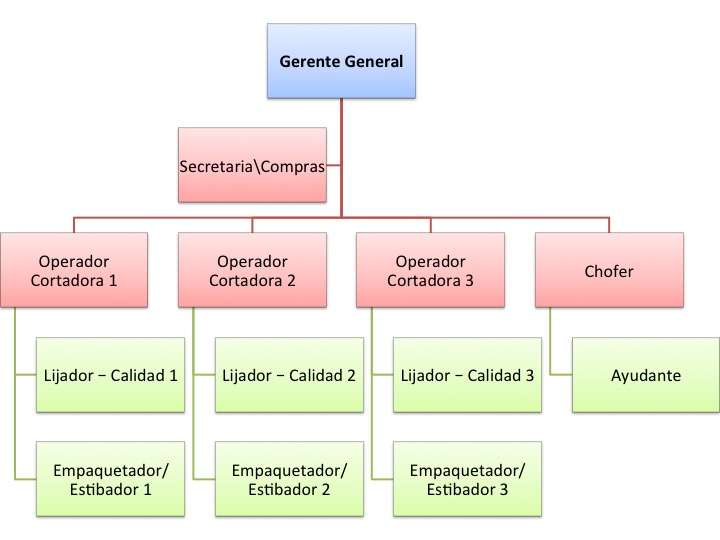
\includegraphics[width=1\textwidth]{Organigrama.jpg}
 \captionsetup{justification=centering} %Centrar caption 
 \caption{Organigrama General}
 \label{figura:4}
\end{figure}

\subsubsection {Sistemas de información}
Como sistema de información la empresa presenta un esquema simple pero que ha resultado útil hasta la fecha.

\begin{itemize}	
		\item Servicio de correo electrónico corporativo
		\item Servicio de telefonía fijo
		\item Servicio de telefonía celular
		\item Software para control de accesos/salidas a la empresa.
	\end{itemize}
Los archivos de la empresa se encuentran respaldados de forma física.

\subsubsection{Infraestructura tecnológica}
Las comunicaciones internas se las realiza mediante telefonía móvil uso de mensajería de instantánea a través de smartphones combinado con teléfonos fijos. El personal administrativo posee un computadora personal con un sistema operativo actualizado.

La empresa posee un camión de 10 Ton utilizado para las entregas de volumen grande y una camioneta para entregas pequeñas. 

Para el control de ingreso y salidas del las áreas de trabajo la empresa posee un lector de huellas digitales que proporciona la llegada y salida de los colaboradores.


\newpage
\section{Caso del Negocio}
\subsection{Resumen Ejecutivo}
\subsubsection{Definición del problema}

La empresa Servimaderas tuvo un crecimiento constante desde su creación lo cual ha permitido  ir incrementando su gama de productos y servicios. Actualmente la empresa enfrenta varios problemas siendo los principales un incremento de los costos de fabricación debido a que tanto la maquinaria como el espacio físico se encuentran subutilizados lo cual se ha hecho mas evidente debido a que ha existido una reducción de la participación de mercado en el último año con una disminución de los ingresos que genera la compañía. 

Los ingresos provenientes de la venta de partes y piezas han tenido un decrecimiento constante desde inicios del año 2016 perdiendo a su cliente principal y reduciendo la producción en comparación al año 2015. Mientras que los ingresos por el servicio de secado de madera se ha reducido de manera drástica debido a la apertura del Innovacentro de la Madera y el Mueble en la cuidad de Cuenca la cual ofrece servicios similares. De esta manera la empresa atraviesa un periodo difícil el cual de no sobrepasar puede ocasionar el cierre de la empresa. 

Ante estos factores la empresa requiere recuperar , obtener y mantener clientes de tal forma que sus ingresos permitan la sostenibilidad. De la misma manera es necesario reducir gastos de producción y gestionar de mejor manera el uso de los equipos y materiales a fin de tener productos y servicios eficientes y ser mas competitivos ante los diferentes competidores.

\subsubsection{Análisis de Brechas}
A partir del análisis de las estrategias y la arquitectura empresarial todo esto enfocando  a resolver el problema definido el cual se basa en la reducción de ventas desde el año 2016 y la reducción de servicios prestados ; sumado a una baja eficiencia en sus procesos de producción  ha permitido  identificar  brechas y necesidades las cuales se relacionan con las iniciativas de manera que se busca establecer cuales son las iniciativas que  resuelven las brechas y que necesidades son satisfechas. Este análisis se presenta en  Tabla \ref{brechas}. 

\begin{table}[H]
\centering
\caption{Brechas, necesidades e iniciativas }
\label{brechas}
\begin{tabular}{|p{5cm}|p{5cm}|p{4cm}|}
\hline
\multicolumn{1}{|c|}{\textbf{Brechas}} & \multicolumn{1}{c|}{\textbf{Necesidades}} & \multicolumn{1}{c|}{\textbf{Iniciativas}} \\ \hline
Espacio físico y equipo subutilizado & Aumentar eficiencia en producción & \multirow{3}{4cm}{\\Implementar procesos estandarizados de producción} \\ \cline{1-2}
Falta de procesos estandarizados reduce eficiencia & Optimizar tiempos de producción &  \\ \cline{1-2}
Cultura organizacional enfocada a cantidad de producción y no a eficiencia de recursos & Reducir desperdicios de materias primas &  \\ \hline
Participación reducida en el mercado provincial. & Incrementar volumen de ventas en productos y servicios & \multirow{3}{4cm}{\\Implementar una producción eficiente mediante diversificación de portafolio y apertura de nuevos mercados} \\ \cline{1-2}
Uso deficiente del espacio y maquinaria & Mejorar el uso de los recursos de la empresa &  \\ \cline{1-2}
Falta de diversidad de productos para otros segmentos & Elaborar nuevos productos &  \\ \hline
Falta de sistema de control de reclamos del cliente & Ofrecer atención a reclamos de manera oportuna & Establecer sistema de control de reclamos \\ \hline
Falta de planes de capacitación para el personal interno & Personal capacitado para las actividades & \multirow{4}{4cm}{Realizar procesos de evaluación al personal} \\ \cline{1-2}
Falta de métodos de evaluación de desempeño & Controlar el desempeño de los recursos dentro del proceso &  \\ \cline{1-2}
Falta de métodos de reconocimiento a los colaboradores & Generar compromiso de los colaboradores con la empresa &  \\ \cline{1-2}
Falta de métodos de control de la producción & Establecer métricas de producción &  \\ \hline
\end{tabular}
\end{table}




\subsubsection{Iniciativas Claves}
En la  Tabla \ref{Priorizacion:Iniciativas} se priorizan las iniciativas obtenidas mediante el análisis realizado en la Tabla \ref{Iniciativas} a través de definir la urgencia que se tiene por la implementación y el impacto económico que cada iniciativa posee. Se considera una puntuación que va desde 1 como Bajo y 3 como Alto. La prioridad se obtiene mediante el producto de la urgencia y el impacto este método es cualitativo y busca priorizar las iniciativas que se realizaran.

\begin{table}[H]
\centering
\caption{\textit{ Priorización de iniciativas} }
\label{Priorizacion:Iniciativas}
\begin{tabular}{|p{5cm}|l|l|l|}
\hline
\textbf{Iniciativa} & \textbf{Impacto} & \textbf{Urgencia} & \textbf{Prioridad} \\ \hline
Implementar una producción eficiente mediante diversificación de portafolio y apertura de nuevos mercados & 3 & 3 & 9 \\ \hline
Establecer sistema de control de reclamos & 1 & 2 & 3 \\ \hline
Implementar procesos estandarizados de producción & 2 & 3 & 6 \\ \hline
Realizar procesos de evaluación al personal & 1 & 1 & 1 \\ \hline
\end{tabular}
\end{table}

Una vez analizada la matriz se ve que la iniciativa con mayor  prioridad es Implementar una producción eficiente mediante diversificación de portafolio y apertura de nuevos mercados de productos con un puntaje de 9. Para desarrollar esta iniciativa se establecen tres posibles soluciones que se son:

\begin{itemize}
\item Implementación de una línea de producción de muebles en la fábrica Servimaderas.
\item Implementación de sistemas de estandarización del proceso productivo con nuevos productos de partes y piezas.
\item Implementar un sistema de ventas mas agresivo de partes y piezas a empresas que fabriquen muebles a nivel nacional.
\end{itemize}



\end{document}







